%%%%%%%%%%%%%%%%%%%%%%% file template.tex %%%%%%%%%%%%%%%%%%%%%%%%%
%
% This is a template file for Web of Conferences Journal
%
% Copy it to a new file with a new name and use it as the basis
% for your article
%
%%%%%%%%%%%%%%%%%%%%%%%%%% EDP Science %%%%%%%%%%%%%%%%%%%%%%%%%%%%
%
%%%\documentclass[option]{webofc}
%%% "twocolumn" for typesetting an article in two columns format (default one column)
%
\documentclass{webofc}
\usepackage[varg]{txfonts}   % Web of Conferences font

% \usepackage{natbib}
%
% Put here some packages required or/and some personnal commands
%
%
\begin{document}
%
\title{Review of smoothing methods for enhancement of noisy data from heavy-duty LHD mining machines}
%
% subtitle is optionnal
%
%%%\subtitle{Do you have a subtitle?\\ If so, write it here}

\author{\firstname{Jacek} \lastname{Wodecki}\inst{1}\thanks{\email{jacek.wodecki@pwr.edu.pl}} \and
        \firstname{Anna} \lastname{Michalak}\inst{2}\ \and
        \firstname{Paweł} \lastname{Stefaniak}\inst{2}\
        % etc.
}

\institute{Machinery Systems Division, Wroclaw University of Science and Technology, Wroclaw, Poland 
\and
           KGHM Cuprum R$\&$D Ltd., Wroclaw, Poland}

\abstract{%
  Appropriate analysis of data measured on heavy-duty mining machines is essential for processes monitoring, management and optimization. Some particular classes of machines, for example LHD (load-haul-dump) machines, hauling trucks, drilling/bolting machines etc. are characterized with cyclicity of operations. In those cases, identification of cycles and their segments or in other words – simply data segmentation is a key to evaluate their performance, which may be very useful from the management point of view, for example leading to introducing optimization to the process. However, in many cases such raw signals are contaminated with various artifacts, and in general are expected to be very noisy, which makes the segmentation task very difficult or even impossible. To deal with that problem, there is a need for efficient smoothing methods that will allow to retain informative trends in the signals while disregarding noises and other undesired non-deterministic components. In this paper authors present a review of various approaches to diagnostic data smoothing. Described methods can be used in a fast and efficient way, effectively cleaning the signals while preserving informative deterministic behaviour, that is a crucial to precise segmentation and other approaches to industrial data analysis.
}
%
\maketitle
%
\section{Introduction}
\label{intro}
Load-Haul-Dump machines (LHD) are common assets used for ore transportation in production area of a mine with room-and-pillar system. Their character of the work seems very simple – machine loads blasted ore in mining face using bucket, next transports it to dumping point where dumps material onto conveyor belt, and finally returns to the mining face with empty bucket. Each of these sub-processes often differs from cycle to cycle and, consequently, takes up more or less time according to operating conditions in production area \cite{gustafson2013influence}. Depending on length of haulage route LHD machine may work alone as well as may operate in the configuration with haul truck. 

Assessment of LHD machine is crucial from view point of production planning and optimization of haulage of ore from production areas \cite{cui2013production,gustafson2014development}. In the literature, this subject is well-known – in global mining, monitoring solutions are used on a large scale for tracking machine operating parameters, both for efficiency and damage detection \cite{wylomanska2015analysis,wylomanska2014signal,gajda2016subordinated,wodeckicondition}. Algorithms for identification of haulage sub-processes are also developed for both LHD and haul truck. In practice, it is still needed to develop a comprehensive algorithm for operating cycles identification \cite{stefaniak2015effectiveness, mpolak}. Arguably, the easiest way is the analysis of the most informative signals acquired from the machine. 

One of the most interesting signals in terms of its cyclic structure is the pressure signal measured
at a bucket’s hydraulic cylinder. From view point of recognition of LHD's operations pressure signal is much more informativeness than signal of bucket weight mesured when bucket is raised to unload material \cite{stefaniak2016multidimensional}. High and low levels of pressure indicate driving with full or empty bucket. It is even possible to notice the underlying tasks of loading and unloading. Such signal is unfortunately highly contaminated with noise as well as fluctuations coming from the fact that the bucket, either full or empty, is prone to wobbling when the machine is moving, very often while driving on uneven surfaces. Considering described facts, it can be said that the first task required for any algorithm for analysis of the operational cycles is smoothing out the raw signal while preserving its informative structure.
In this paper authors compare the performance of six basic smoothing methods for real-life signal denoising and presents the segmentation based of them.

\section{Methodology}
Signal smoothing can be realized using many different techniques, e.g.: filtering using lowpass or custom filters \cite{mitra2006digital}, additive smoothing \cite{valcarce2016additive}, kernel smoothing \cite{friedman2001elements} or many others. In this paper six methods are compared in terms of quality of denoised signal defined as a readiness for the segmentation, which is the next step in processing of such signals.

\textbf{Moving average (MA)} is one of the most popular methods for smoothing a series of data. It creates a series of average values of the consecutive subsets of the entire dataset. This is a special case of a finite impulse response filter (FIR), where the weights carry the same value of 1/N, where N is the length of the window. \textbf{Exponential moving average (EMA)} is a special case of moving average where weighting factors decrease exponentially \cite{hunter1986exponentially}.

Next group of methods is local regression. In \textbf{linear regression} each smoothed value is determined relative to the neighbouring data samples in a given window based on linear function models \cite{cleveland1996smoothing}. Analogously, \textbf{quadratic regression} smoothed each value based on quadratic model. These two methods have also \textbf{robust versions}, which are very helpful if smoothed data contains outliers. The robust procedure for linear and quadratic regression is given by \cite{cleveland1979robust}:

\begin{enumerate}
    \item Calculate the residuals from the regression smoothing method,
    \item Compute the robust weights for each data point in the window. These weights are defined by:
 \begin{equation}
 w_i =
  \begin{cases}
    $$\left( 1-\left( \frac{r_i}{6MAD} \right)^2 \right)^2$$,    & \quad |r_i| \leq 6MAD\\
    0,  & \quad |r_i| \geq 6MAD,\\
  \end{cases}
 \end{equation}       
 
    where $r_i$ is the residual of $i^{th}$ data point and MAD is the median absolute deviation of the whole window, MAD=median(|r|). If $r_i$ is greater than 6MAD, assigned weight is zero and this data point is excluded from the calculation in next iteration. If the $r_i$ is small compared to 6MAD, then the weight is close to 1.
    \item Repeat steps 1-2 for a total of five iterations,
    \item Smooth data using the robust weights.
\end{enumerate}

\section{Application to real-life data}


Machine investigated in this paper is a self-propelled wheel loader operated in one of the Polish copper ore underground mines for loading, hauling and dumping purposes (see Fig. \ref{LHD_machine}). Total time of loader operations in production area lasts 4-shift work a day (6 hours per shift). Loaders operate in this mode 6 days a week with the exception of short intermissions for maintenance or repair tasks. Total distance of haulage -- defined as route from mining face to dumping point -- does not exceed 800 meters. For some longer distance routes, loaders are intended for filling cargo boxes of haul trucks. All sub-processes are performed in cyclic way.

\begin{figure}[ht!]
% Use the relevant command for your figure-insertion program
% to insert the figure file.
\centering
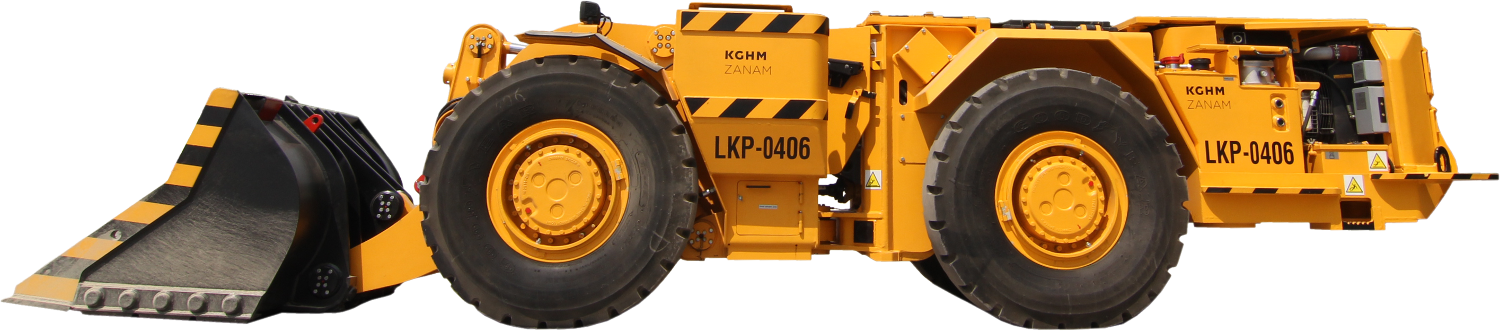
\includegraphics[width=0.7\textwidth,clip]{loader_fig}
\caption{Load-Haul-Dump machine (LHD)}
\label{LHD_machine}       % Give a unique label
\vspace*{-0.7cm}
\end{figure}

As mentioned above, typical LHD machine work in production area consists of a few operation regimes:

\begin{itemize}
    \item   loading of the blasted ore in mining face,
    \item haulage to the dumping point (full bucket),
    \item   unloading onto screen,
    \item returning to mining face (empty bucket).
\end{itemize}


\begin{figure}[ht!]
% Use the relevant command for your figure-insertion program
% to insert the figure file.
\centering
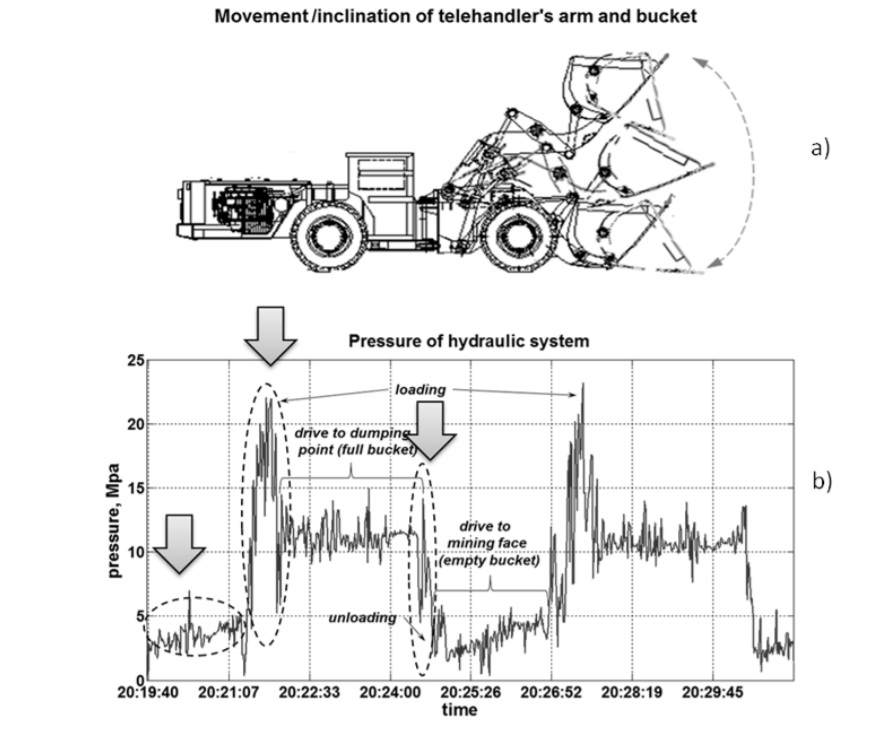
\includegraphics[width=0.6\textwidth,clip]{fig}
\caption{Swing angle of loader’s arm and bucket (panel a) and variability of pressure of hydraulic system during different loader operations (panel b)}
\label{subplot_machine_signal}       % Give a unique label
\vspace*{-0.7cm}
\end{figure}




Each of these haulage sub-processes corresponds to different inclination of telehandler’s arm as well as filling of the bucket (see Fig. \ref{subplot_machine_signal}a). These two features appear in the hydraulic pressure signal in form of specific pattern (see Fig. \ref{subplot_machine_signal}b). The high values of pressure with high fluctuations are responsible for loading process. Next, the signal is stabilising on around 12 MPa what indicates transport of the ore to the dumping point. Then, the rapid drop of pressure value is observed during unloading of bucket onto screen. After that, in last phase the LHD machine returns to mining face. Loader is driving the same route back with empty bucket and hydraulic pressure has settled low value.

\subsection{Input data}

Raw signal considered here consists of 280 minutes time series representing pressure in hydraulic system of loader under its typical load-haulage-dump operations (see Fig. \ref{surowe}). The signal has been acquired using bulit-in data acquisition system. On-board monitoring system records operating data with sampling period of 1 second. Data describes period of single work-shift of LHD machine.

\begin{figure}[ht!]
% Use the relevant command for your figure-insertion program
% to insert the figure file.
\centering
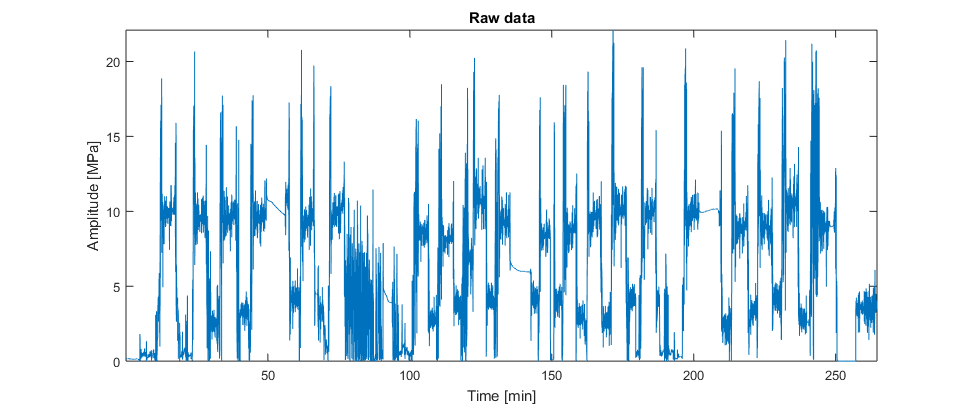
\includegraphics[width=0.95\textwidth,clip]{raw_data}
\caption{Raw data}
\label{surowe}       % Give a unique label
\vspace*{-0.8cm}
\end{figure}

\subsection{Results}

As a first step, presented input signal has been processed with all described methods. Since all methods use window length as a parameter, the same value of 61 samples has been provided not only for reliable comparison, but also due to the fact that it turned out to be optimal value for all of the methods individually.

\begin{figure}[ht!]
% Use the relevant command for your figure-insertion program
% to insert the figure file.
\centering
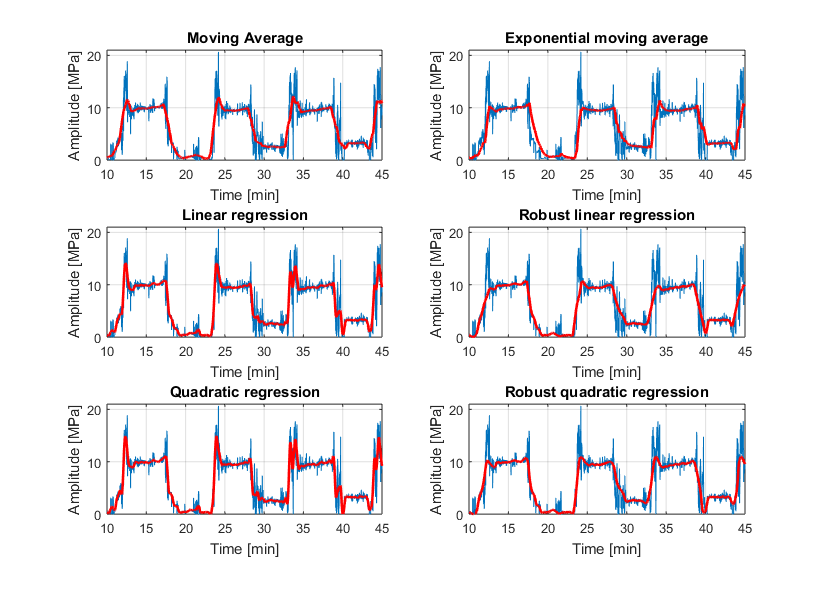
\includegraphics[width=0.8\textwidth,clip]{ladne}
\vspace*{-0.8cm}
\caption{Signal section presenting typical behavior}
\label{ladne}       % Give a unique label
\vspace*{-0.8cm}
\end{figure}
% \vspace*{-1cm}

Figure \ref{ladne} presents results of smoothing with all methods using only a section where behavior of input signal was very much typical, operational cycles looked undisturbed and similar to each other. Such signal shape is expected when machine operates normally, without any disturbances. One can see a clear difference between results produced with tested smoothing methods. 

Both moving average methods as well as both robust regression algorithms produced signals similar to a square wave, without very significant distinction of loading section in the beginning of the high state of the signal. They appear to be a good foundation for further segmentation. On the other hand both of basic regression methods provide more detail and precision for the loading section, and for the shape of entire signal.

\begin{figure}[ht!]
% Use the relevant command for your figure-insertion program
% to insert the figure file.
\centering
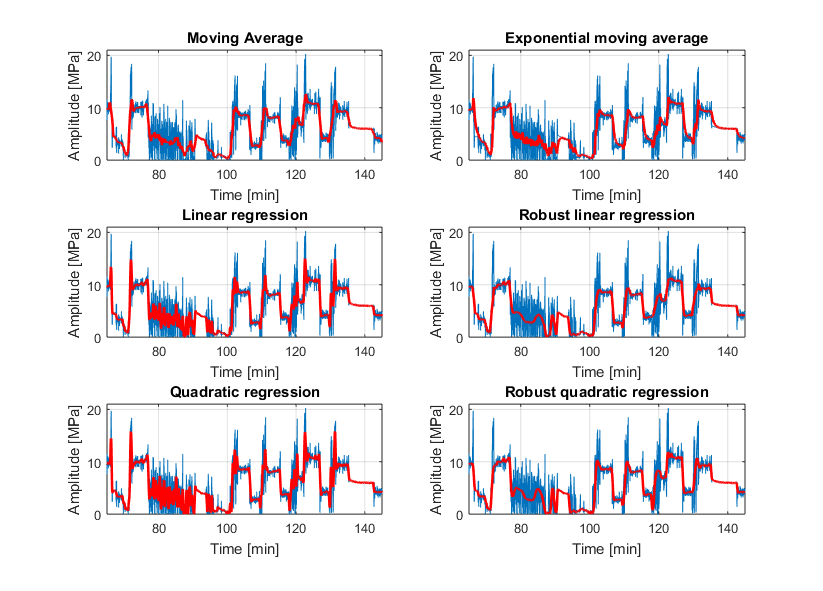
\includegraphics[width=0.8\textwidth,clip]{brzydkie}
\vspace*{-0.8cm}
\caption{Signal section presenting anomalies and occasional alterations of typical behavior}
\label{brzydkie}       % Give a unique label
\vspace*{-0.8cm}
\end{figure}
% \vspace*{-1cm}

Figure \ref{brzydkie} presents results of smoothing with all methods, this time presented with a section containing non-typical events, e.g. fast oscillations between $75^{th}$ and $100^{th}$ minute, that may indicate other type of activity, extended loading action around $120^{th}$ minute or stoppage around $140^{th}$ minute. Such cases can translate into unpredictable effects of threshold-based segmentation and are key aspects for smoothing performance evaluation.

\begin{figure}[ht!]
% Use the relevant command for your figure-insertion program
% to insert the figure file.
\centering
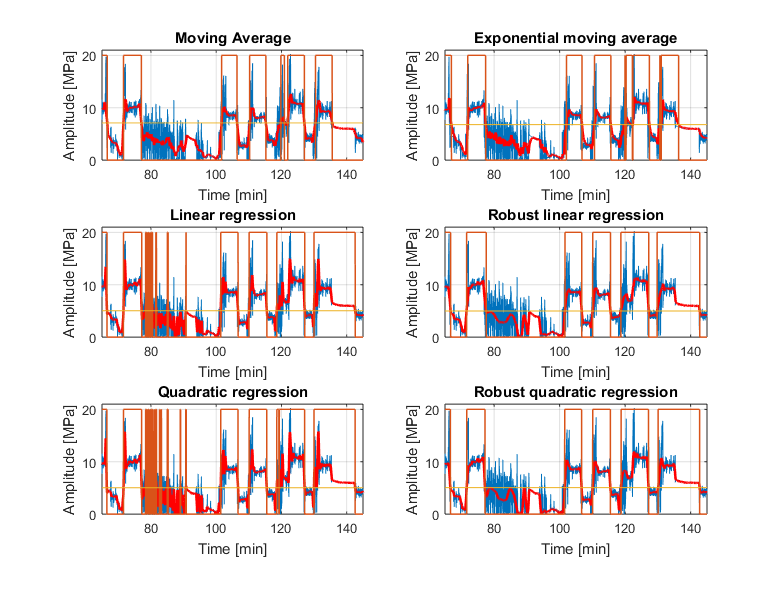
\includegraphics[width=0.8\textwidth,clip]{bseg}
\vspace*{-0.8cm}
\caption{Non-typical signal section with segmentation results and threshold level}
\label{bseg}       % Give a unique label
\vspace*{-0.8cm}
\end{figure}

Such segments especially visualize major differences between smoothing results. Again, basic regression methods appear to produce the most details, which can be misleading for segmentation procedure. Other methods produce smoother results with robust regression methods appearing to be the least jagged in details.

Figure \ref{bseg} presents results of segmentation of smoothed signals. Segmentation is based on separating signal values above and below certain automatically calculated threshold, which is obtained as a central point of signal histogram (see Figure \ref{hist}). It is identified as an average of two maim local maxima obtained after splitting the histogram in half according to amount of samples. Quantitative factor of smoothing quality is here expressed as a percentage of known cycles amount identified by segmentation. 

As it can be seen in Table \ref{tab-1} basic linear regression methods are characterized with the worst quality, which is also visible in Figure \ref{bseg}. In those cases segmentation detects a lot of unnecessary cycles in the areas of unexpected events. Both moving average methods perform better, but they still detect some extra cycles, e.g. when the extended loading action occurs around $120^{th}$ minute. They are also having problem with spanning the cycles in a correct way. When the stoppage occurs around $140^{th}$ minute, MA methods close the cycle just before the stoppage, in contrast to the basic or robust regression methods, that capture this cycle correctly, according to the experts of LHD machines' operation. 

\begin{table}[ht!]
\centering
\caption{Results of segmentation based on denoised signals}
\label{tab-1}       % Give a unique label
% For LaTeX tables you can use
\begin{tabular}{lll}
\hline
Method & Number of cycles & Percentage  \\\hline
Known amount & 20 & 100$\%$ \\
Moving Average & 21 & 105$\%$ \\
Exp. Moving Average & 23 & 115$\%$ \\
Linear Regression & 29 & 145$\%$ \\
Robust Linear Regression & 20 & 100$\%$ \\
Quadratic Regression & 34 & 170$\%$ \\
Robust Quadratic Regression & 20 & 100$\%$ \\\hline
\end{tabular}
% Or use
% \vspace*{5cm}  % with the correct table height
\end{table}

\begin{figure}[ht!]
% Use the relevant command for your figure-insertion program
% to insert the figure file.
\centering
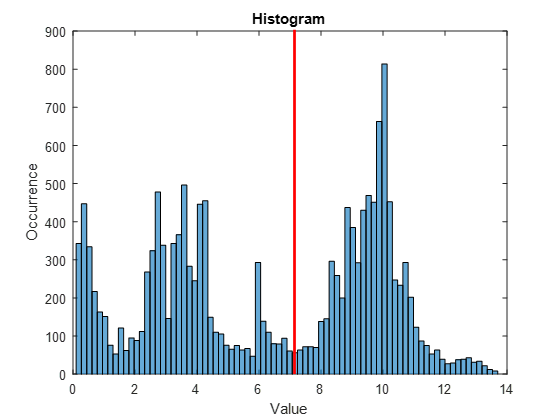
\includegraphics[width=0.6\textwidth,clip]{hist}
\caption{Example of histogram-based thresholding method. Threshold value is calculated as central point of histogram constructed from smoothed signal}
\label{hist}       % Give a unique label
\vspace*{-0.8cm}
\end{figure}

Finally, robust regression methods appear to perform as perfectly as it is possible for such type of data. They identify correct amount of cycles in the whole signal, and questionable cycles are captured in a correct way. Namely, cycle containing extended loading action should be captured as a whole, along with the early phase of loading, as well as cycle containing stoppage should also be captured as a whole.

It is very important to note that one could easily implement security measures to avoid capturing too short cycles, which would eliminate excessive amount of cycles to the point when all of the methods would result in correct number of detected cycles. Although there are two points to be made in this matter:

\begin{enumerate}
    \item As it can be seen in Figure \ref{bseg} even after cleaning up short cycles, it is still important to properly capture correct cycles (see cycle with the stoppage),
    \item The point of presented comparison is to verify which method can function properly without need to implement additional verification procedures. It is very important for final implementations in analytical systems to minimize the amount of additional procedures.
\end{enumerate}

Taking those points into consideration, it can be summarized that robust regression methods are the best solutions for preprocessing similar types of signals. Additionally, since those methods focus on outliers analysis, it can be said that this aspect is very important while taking any smoothing actions.

\section{Conclusions}

Signals measured in underground mine reality are particularly susceptible to interference, which very often reduces the level of their informativeness, and this in turn might lead to wrong interpretation of the analysis results. The reasons for this are partly to be found in harsh mining conditions where machines operate in a cyclic way and their work consists of many sub-processes. In practice, there exist many ways to improve quality of measured signals commonly used at pre-processing level. In this paper, authors focused on review of smoothing methods for further segmentation of pressure signal in terms of further identification of work cycles of LHD machine. In fact, pressure signal measured at a bucket's hydraulic cylinder is very regular and at first glance seems like square wave clearly defined two main sub-processes of ore haulage (driving with full and empty bucket). Although, because of high fluctuations and noise level, it is not possible to detect a regime changes based on raw signal. Presented paper compares six smoothing methods in terms of readiness to segment smoothed signal produced by them. Extensive testing showed that robust regression methods perform the best in such application.

%
% BibTeX or Biber users please use (the style is already called in the class, ensure that the "woc.bst" style is in your local directory)
% \bibliography{name or your bibliography database}
%
% Non-BibTeX users please use
%
% \bibliographystyle{woc}
\bibliography{mybib}
% \begin{thebibliography}{}
% % and use \bibitem to create references.
% \bibitem{mitra2006digital}
% S.K. Mitra, \textit{Digital Signal Processing: A Computer-Based Approach}, New York, NY: McGraw-Hill (1998)
% \bibitem{RefJ}
% % Format for Journal Reference
% Journal Author, Journal \textbf{Volume}, page numbers (year)
% % Format for books
% \bibitem{RefB}
% Book Author, \textit{Book title} (Publisher, place, year) page numbers
% % etc
% \end{thebibliography}

\end{document}
